\section{Preferences}
The preference system allows the user to change settings which are otherwise not accessible. An example would be the shortcut for maximizing a \src{Dockable} (\src{ctrl+m}). The preference system makes a sharp distinction between model and view, clients are free to integrate the model in their own view, or to create a new model and using the standard view. Figure \ref{fig:preferences} shows the simple version of the standard view with some random preferences.

\begin{figure}[ht]
\centering
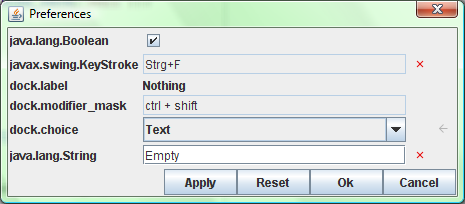
\includegraphics[width=0.5\textwidth]{preferences/preferences}
\caption{The \src{PreferenceDialog} showing some random preferences.}
\label{fig:preferences}
\end{figure}

Additionaly the prerefence API offers mechanism to persistently store preferences.

\subsection{Model}
The model is an adapter to the view and presents some properties as a list of modifiable items. Whether the model represents properties of the framework or custom properties is unimportant for the view or the persistent storage mechanism to work.

\subsubsection{Preference}
A preference is an abstract concept. One preference represents some property of the framework (or of the client). A preference is a set of meta-informations about a property:
\begin{description}
 \item[Path] A unique identifier, is used by the persistent storage to identify a property.
 \item[Value] The current value of the property.
 \item[TypePath] Tells how to work with \src{Value}. For example how to present the value to the user (as text, as image...) or how to store the value. An object of type \src{Path} is used to represent the \src{TypePath}.
 \item[ValueInfo] Information about the value, e.g. the maximum value for an \linebreak \src{Integer}-property. The exact meaning of this information depends on the \src{TypePath}.
\end{description}

\designbox{\src{Value} is some \src{Object} and \src{TypePath} tells the view how to cast \src{Value} in order to use it. If \src{TypePath} were a \src{Class} then there would never be doubt whether the correct cast is performed. But \src{TypePath} is a \src{Path} and hence an additional indirection is introduced.

The reason for this is that the same \src{Object} might need different treatment in different situations. E.g. an \src{Integer} could just be an int, it could be a natural number or it could be an int from the range 1 to 100.}

\classbox{There is an interface \src{Preference} and a class \src{DefaultPreference} which bring this preference-abstraction to code. It is not necessary to use them, they are just here to simplify things.}

\subsubsection{PreferenceModel}
The \src{PreferenceModel} is the basic module of the preference system. A \linebreak \src{PreferenceModel} is a list of preferences (the abstraction, not the interface). It often acts as mediator between some unspecified storage mechanism for properties and the user interface. The methods \src{read} and \src{write} are used to access that covered storage mechanism. To transfer values into the model \src{read} is called, to transver values to the storage mechanism \src{write} is called.

\classbox{\src{DefaultPreferenceModel} is the standard implementation of \src{PreferenceModel}. Its entries are objects of type \src{Preference}.

Several models can be combined using a \src{MergedPreferenceModel}.}

\infobox{There are several subclasses of \src{DefaultPreferenceModel} for various settings that can be made. For example \src{EclipseThemeModel} handles properties of \src{EclipseTheme}.

There are also many implementations of \src{Preference} for various properties of the framework. The API-documentation reveals more.}

\subsubsection{PreferenceTreeModel}
This model is a \src{PreferenceModel} and a \src{javax.swing.TreeModel}. If seen as \src{PreferenceModel}, then it behaves like a \src{MergedPreferenceModel}. If seen as \src{TreeModel}, then it contains \src{PrefereceTreeModel.Node}-objects. A node can either be just a name, or another \src{PreferenceModel}. This model is intended to be used in a \src{JTree} where the user can select one aspect of the whole set of preferences to show.

\classbox{The subclass \src{DockingFramesPreferenceModel} is the set of preferences which includes all the aspects of the core-library.}

\subsection{View}
A \src{PreferenceModel} is best displayed in a \src{PreferenceTable}. This table will show a label, an editor and operations for each preference. 

A \src{PreferenceTreeModel} can be displayed in a \src{PreferenceTreePanel}. It will show not only a \src{PreferenceTable} but also a \src{JTree} where the user can select which sub-model to edit.

Further more the \src{PreferenceDialog} and the \src{PreferenceTreeDialog} are available. These dialogs offer the options to apply the settings, to cancel editing and to reset all preferences to their default value.

\subsubsection{Editors}
Since there are different types of preferences, different editors are needed. The kind of editor for one preference is determined by the type-path (\src{getTypePath} in a model). Clients can add new editors to a \src{PreferenceTable} through the method \src{setEditorFactory}.

An editor is always of type \src{PreferenceEditor}. Each editor gets a \linebreak \src{PreferenceEditorCallback} with which it can interact with the table. Whenever the user changes the editors value, the editor should call the method \src{set} of \src{PreferenceEditorCallback} to make sure the new value gets stored.

\subsubsection{Operations}
There are some operations which should be available for almost any preference. For example \textit{set a default value} or \textit{delete the current value}. The preference system introduces the \src{PreferenceOperation} to handle these kind of actions.

A \src{PreferenceOperation} is nothing more than a label and an icon. The logic for an operation is either in an editor or in a model.

\begin{description}
 \item[Editor:] Editors with operations must call the method \src{setOperation} of \linebreak \src{PreferenceEditorCallback} for each operation they offer. By calling \src{setOperation} more than once, the editor can change the enabled state of the operation. If the user triggers an operation of the editor, the method \src{doOperation} of \src{PreferenceEditor} is called. It is then the editors responsibility to handle the operation.
 \item[Preference:] Preferences can have operations as well. The method \linebreak \src{getOperations} of \src{PreferenceModel} will be called once to get all the available operations for one preference. The method \src{isEnabled} will be invoked to find out whether an operation is enabled or not. Models can change the enabled state by calling \src{preferenceChanged} of \linebreak \src{PreferenceModelListener}. If the user triggers an operation, \linebreak \src{doOperation} of \src{PreferenceModel} will be invoked.
\end{description}
If an editor and a preference share the same operations, then per definition the operations belong to the editor. All settings from the model will just be ignored.

\infobox{Operations might be confusing at first, but they can be really useful. The strength of operations is that they are handled automatically, and that they need not much code.}

\subsection{Storage}
The \src{PreferenceStorage} can be used to store \src{PreferenceModel}s in memory or persistent either as byte-stream or as XML.

The normal way to write a model from memory to the disk looks like this:
\begin{lstlisting}
// the stream we want to write into
DataOutputStream out = ...

// the model we want to store
PreferenceModel model = ...

// And now store the model
PreferenceStorage storage = new PreferenceStorage();
storage.store( model );
storage.write( out );
\end{lstlisting}
Note that there are two phases in writing \src{model}. First the model gets \src{store}d (line \src{9}) into \src{storage}. It is possible to store more than just one model in a \src{PreferenceStorage}. Second \src{storage} gets written onto the disk in line \src{10}.

The standard way to read a model are to apply the same steps in reverse:
\begin{lstlisting}
// the source of any new data
DataInputStream in = ...

// the model we want to load
PreferenceModel model = ...

// And now load the model
PreferenceStorage storage = new PreferenceStorage();
storage.read( in );
storage.load( model, false );
\end{lstlisting}
Like writing this operation has two phases. In line \src{9} \src{storage} gets filled with information, in line \src{10} the information gets transfered to \src{model}. The argument \src{false} is a hint what to do with missing preferences. In this case missing preferences are just ignored. A value of \src{true} would force them to become \src{null}.

There are some preferences which do not need to be stored by the \linebreak \src{PreferenceStorage} because they are already stored by the underlying system. These preferences are called \textit{natural}, while the others are called \textit{artificial}. The method \src{isNatural} of \src{PreferenceModel} can be used to distinguish them.

\designbox{The distinction between natural and artificial preferences might seem curious. But actually this allows to use an unlimited number of storage mechanisms at the same time.}

\subsection{Lifecycle}
This section describes the best way how to use a \src{PreferenceModel}.

The correct lifecycle of a \src{PreferenceModel} includes normally these steps:
\begin{enumerate}
 \item Create the model. Set up all the preferences that are used by the model.
 \item Call \src{load} on a \src{StoragePreference}.
 \item Call \src{write} on the model to synchronize the model with the underlying system.
 \item (work with the underlying system)
 \item To work with the model: call first \src{read}, then make the changes in the model, then call \src{write}.
 \item (work with the underlying system)
 \item Call \src{read} on the model to synchronize the model with the underlying system.
 \item Store the model using \src{store} of a \src{PreferenceStorage}.
\end{enumerate}

If the \src{PreferenceStorage} used in step \src{2} is empty because its \src{read} or \src{readXML} method failed, then calling \src{read} of \src{PreferenceModel} would at least load some default settings.

Steps \src{4, 5, 6} can be cycled as many times as needed.

An additional step \src{0} and \src{9} would be to read and write the \\\src{PreferenceStorage} when starting up or shuting down the application.